% Broadband Expansion and Small-Firm Productivity — 30-minute author talk.
% Source: the fictional demonstration manuscript linked from README.md.
\documentclass[11pt,aspectratio=169]{beamer}
\usepackage{econ-slides-house}
% Shared title metadata and source-traceable result phrases for the deck/script.
\newcommand{\PaperTitle}{Broadband Expansion and Small-Firm Productivity}
\newcommand{\PaperSubtitle}{Evidence from a Staggered Municipal Rollout}
\newcommand{\PaperFullTitle}{\PaperTitle: \PaperSubtitle}
\newcommand{\PaperShortTitle}{Broadband and Small-Firm Productivity}
\newcommand{\PaperAuthors}{Astrid Lindqvist \and Tomas Berg}
\newcommand{\ScriptAuthors}{Astrid Lindqvist and Tomas Berg}
\newcommand{\AuthorShort}{Lindqvist and Berg}
\newcommand{\VenueDate}{July 2026}
\newcommand{\TitleDisclaimer}{Demonstration manuscript; fictional setting and simulated data.}

\newcommand{\ResMunicipalities}{284} % Program description, paper pp. 1 and 4.
\newcommand{\ResFirms}{9{,}400} % Sample construction, paper pp. 1 and 5.
\newcommand{\ResFirmYears}{112{,}800} % Table 1 and sample construction, paper p. 5.
\newcommand{\ResYears}{2008--2019} % Sample construction, paper pp. 1 and 5.
\newcommand{\ResRolloutYears}{2011--2018} % Program description, paper pp. 1 and 4.

\newcommand{\ResBaseline}{0.034} % Table 2, col. (1), paper p. 7; log points.
\newcommand{\ResBaselineSE}{0.002} % Table 2, col. (1), paper p. 7.
\newcommand{\ResControls}{0.033} % Table 2, col. (2), paper p. 7; log points.
\newcommand{\ResControlsSE}{0.002} % Table 2, col. (2), paper p. 7.
\newcommand{\ResTrends}{0.030} % Table 2, col. (3), paper p. 7.
\newcommand{\ResTrendsSE}{0.002} % Table 2, col. (3), paper p. 7.
\newcommand{\ResMunicipalCluster}{0.034} % Table 2, col. (4), paper p. 7.
\newcommand{\ResMunicipalClusterSE}{0.003} % Table 2, col. (4), paper p. 7.

\newcommand{\ResInteractionIntercept}{0.020} % Table 4, col. (1), paper p. 9.
\newcommand{\ResInteractionInterceptSE}{0.003} % Table 4, col. (1), paper p. 9.
\newcommand{\ResInteraction}{0.032} % Table 4, col. (1), paper p. 9.
\newcommand{\ResInteractionSE}{0.005} % Table 4, col. (1), paper p. 9.
\newcommand{\ResCommMean}{0.42} % Table 1, paper p. 5.
\newcommand{\ResCommSD}{0.20} % Table 1, paper p. 5.
\newcommand{\ResCommSDGap}{0.0064} % Derived: 0.032 x 0.20; Tables 1 and 4, pp. 5 and 9.

\newcommand{\ResPlacebo}{-0.004} % Table 3, paper p. 8; log points.
\newcommand{\ResPlaceboSE}{0.002} % Table 3, paper p. 8.
\newcommand{\ResDropEarly}{0.037} % Table 5, col. (3), paper p. 9.
\newcommand{\ResDropEarlySE}{0.002} % Table 5, col. (3), paper p. 9.
\newcommand{\ResPolicyValue}{410 million euros} % Section 7, paper pp. 8--9.
\newcommand{\ResPolicyCost}{2.3 billion euros} % Section 7, paper p. 9.

\newcommand{\ResultHeadlineSlide}{Labor productivity is about 3.4\% higher after backbone availability.}
\newcommand{\ResultHeadlineSpoken}{the same firm produces about 3.4 percent more real value added per worker}
\newcommand{\ResultSupportSlide}{A one-SD increase in communication intensity adds \ResCommSDGap\ log points, about one-fifth of the main difference.}
\newcommand{\ResultSupportSpoken}{a one-standard-deviation increase in communication intensity adds about 0.0064 log points, or one-fifth of the main difference}
\newcommand{\ResultImplicationSlide}{digital infrastructure may matter most where communication frictions bind.}
\newcommand{\ResultImplicationSpoken}{digital infrastructure may matter most where communication frictions bind}


% COLOR MAP (held throughout):
%   broadband availability = teal, matching the source rollout figure
%   communication intensity = blue
\colorlet{cBroadband}{cAccentC}
\colorlet{cTasks}{cAccentA}

\title[\PaperShortTitle]{\PaperTitle:\texorpdfstring{\\[0.25em]}{ }\PaperSubtitle}
\author[\AuthorShort]{\PaperAuthors}
\institute{}
\date{\VenueDate}

\begin{document}

% Exact paper title/subtitle and metadata only, plus the source's disclaimer.
\begin{frame}[plain]
  \titlepage
  \vfill
  \centering\scriptsize\textit{\TitleDisclaimer}
\end{frame}
\addtocounter{framenumber}{-1}

% ---- 1. Key question ----
\begin{frame}{Key question}
  \hypertarget{main:question}{}%
  \medskip
  \KeyIdea{Can \textcolor{cBroadband}{municipal broadband availability} raise small-firm productivity?}

  \bigskip
  \RunIn{Why this matters:}
  \begin{itemize}\setlength{\itemsep}{0.56em}
    \item Small firms adopt new technologies later and less completely
    \item Distance can limit access to specialized providers and inputs
  \end{itemize}

  \bigskip
  \RunIn{Empirical test:}
  \begin{itemize}\setlength{\itemsep}{0.56em}
    \item Is labor productivity higher after \textcolor{cBroadband}{municipal service} arrives?
    \item Is the difference larger for \textcolor{cTasks}{communication-intensive firms}?
  \end{itemize}

  \bigskip
  \textbf{Policy relevance:} whether universal infrastructure changes small-firm production.
\end{frame}

% ---- 2. Punchline ----
\begin{frame}{This paper}
  \hypertarget{main:punchline}{}%
  \medskip
  We link \ResFirms\ firms in \ResYears\ to broadband rollout across
  \ResMunicipalities\ municipalities.
  \bigskip
  \begin{enumerate}\setlength{\itemsep}{1.0em}
    \item \KeyIdea{\ResultHeadlineSlide}
      \vspace{0.16em}
      \begin{itemize}\setlength{\itemsep}{0.42em}
        \item The difference survives firm controls and region-specific trends
      \end{itemize}
    \item \textbf{\textcolor{cTasks}{Communication-intensive firms} show a larger difference.}
      \vspace{0.16em}
      \begin{itemize}\setlength{\itemsep}{0.42em}
        \item One SD adds \ResCommSDGap\ log points, about one-fifth of the main difference
        \item The model links this pattern to the value of remote coordination
      \end{itemize}
  \end{enumerate}

  \bigskip
  \textbf{Implication:} \ResultImplicationSlide
\end{frame}

% ---- 3. Quick roadmap ----
\begin{frame}{Roadmap}
  \begin{enumerate}\setlength{\itemsep}{1.1em}
    \item Setting and data
    \item Design and main evidence
    \item Model and interpretation
  \end{enumerate}
\end{frame}

% ---- 4. Program setting ----
\begin{frame}{Broadband reached every municipality in eight waves}
  \hypertarget{main:rollout}{}%
  \framesubtitle{All \ResMunicipalities\ municipalities connected between \ResRolloutYears}
  \centering
  % Exact crop of paper Figure 1, p. 5; reused without redrawing.
  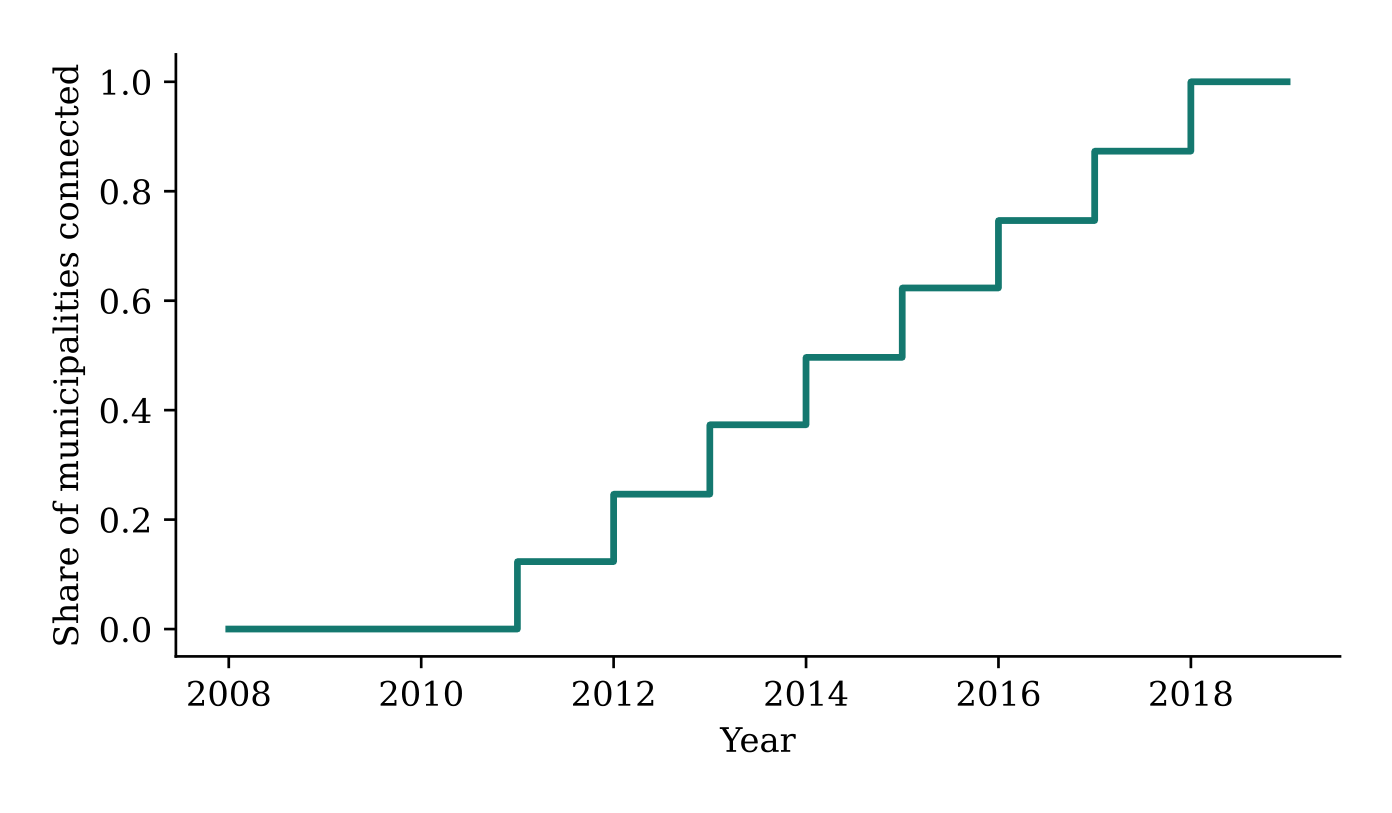
\includegraphics[height=0.62\textheight,keepaspectratio]{figures-slides/fig1_rollout.png}
  \Takeaway{\textbf{Measurement:} exposure begins with municipal service; firm adoption is unobserved.}
\end{frame}

% ---- 5. Data ----
\begin{frame}{Data}
  \hypertarget{main:data}{}%
  \framesubtitle{Business Register, audited accounts, and employer--employee records, \ResYears}
  \begin{itemize}\setlength{\itemsep}{0.78em}
    \item \RunIn{Sample:} \ResFirms\ firms and \ResFirmYears\ firm-years, \ResYears
      \begin{itemize}
        \item 3--49 employees in 2008, positive sales, balanced survivor panel
      \end{itemize}
    \item \RunIn{Outcome:} real value added per worker
      \begin{itemize}
        \item audited accounts deflated by industry prices, divided by FTE employment
      \end{itemize}
    \item \textcolor{cBroadband}{\RunIn{Broadband:}} first commercial-service year in the headquarters municipality
    \item \textcolor{cTasks}{\RunIn{Communication intensity:}} 2008 wage-bill share in communication-intensive jobs
  \end{itemize}
  \PlaceNav{\hyperlink{app:sample}{\beamergotobutton{Sample details}}}
\end{frame}

% ---- 6. Design ----
\begin{frame}{The design follows firms as local backbone service arrives}
  \hypertarget{main:design}{}%
  \framesubtitle{Within-firm comparison across different municipal arrival dates}
  \medskip
  % Baseline specification: paper equation (6), p. 6.
  \[
    y_{it}=\alpha_i+\lambda_t
      +\textcolor{cBroadband}{\beta B_{m(i)t}}
      +X_{it}'\delta+\varepsilon_{it}
  \]
  \begin{itemize}\setlength{\itemsep}{0.68em}
    \item \RunIn{Comparison:} within-firm changes across municipal arrival dates
    \item \RunIn{Fixed effects:} remove permanent firm differences and common year shocks
    \item \RunIn{Counterfactual:} municipalities served at different dates would follow similar paths
    \item \RunIn{Diagnostic:} pre-arrival coefficients test that condition
  \end{itemize}
\end{frame}

% ---- 7. Main estimates ----
\begin{frame}{Labor productivity is about 3.4\% higher after arrival}
  \hypertarget{main:estimates}{}%
  \framesubtitle{Log labor productivity; firm and year fixed effects}
  \centering
  % Exact cells from paper Table 2, p. 7. No paper-table paste.
  {\small\renewcommand{\arraystretch}{1.10}
  \begin{tabular}{lcccc}
    \toprule
      & Baseline & Firm controls & Region trends & Municipal SEs \\
    \midrule
    \textcolor{cBroadband}{Broadband}
      & \textcolor{cBroadband}{\textbf{\ResBaseline***}}
      & \ResControls***
      & \ResTrends***
      & \ResMunicipalCluster*** \\
      & \textcolor{cBroadband}{(\ResBaselineSE)}
      & (\ResControlsSE)
      & (\ResTrendsSE)
      & (\ResMunicipalClusterSE) \\
    Firm and year effects & Yes & Yes & Yes & Yes \\
    Observations & \ResFirmYears & \ResFirmYears & \ResFirmYears & \ResFirmYears \\
    \bottomrule
  \end{tabular}}
  \smallskip

  {\footnotesize SEs are firm-clustered except the final column
  (municipality-clustered); stars reproduce the source.\par}
  \TakeawayWithNav[\ExhibitReadingGapRoomy]{The productivity difference remains about 3\% with firm controls and regional trends.}
  \PlaceNav{\hyperlink{app:sourceconflicts}{\beamergotobutton{Source notes}}\;\hyperlink{app:inference}{\beamergotobutton{Inference}}}
\end{frame}

% ---- 8. Dynamic evidence and the one main caveat ----
\begin{frame}{Productivity rises before and after broadband arrives}
  \hypertarget{main:eventstudy}{}%
  \framesubtitle{Paper Figure 2; $t=-1$ omitted; firm-clustered 95\% intervals}
  \centering
  % Exact crop of paper Figure 2, p. 7; no coefficient is read from pixels.
  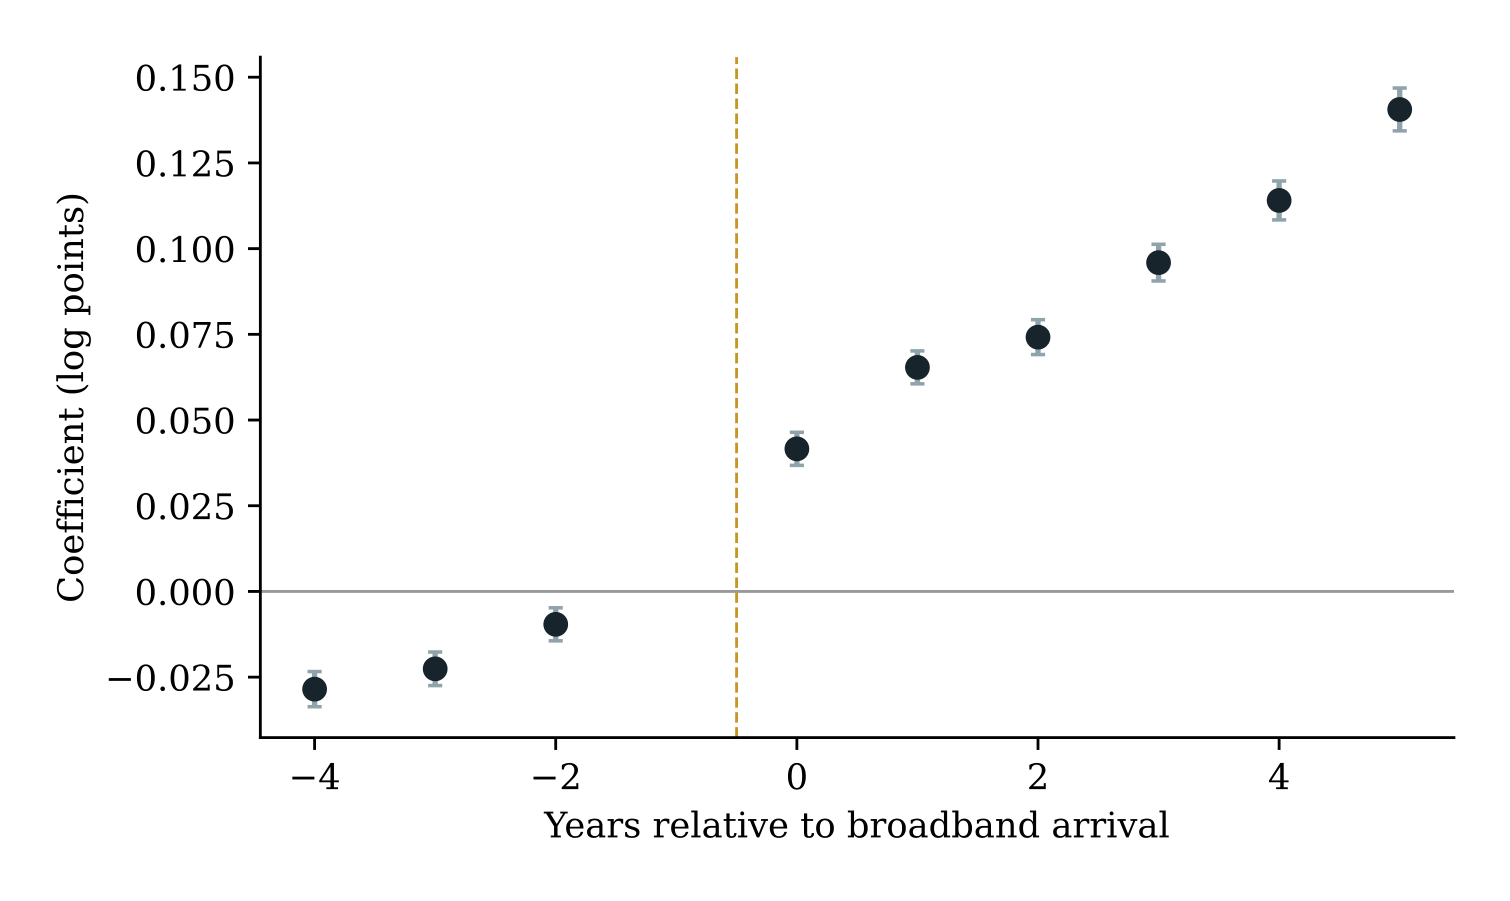
\includegraphics[height=0.60\textheight,keepaspectratio]{figures-slides/fig2_event_study.png}
  \TakeawayWithNav{\textbf{Limitation:} The visible pretrend limits the estimates to a descriptive reading.}
  \PlaceNav{\hyperlink{app:assignment}{\beamergotobutton{Assignment}}\;\hyperlink{app:cohorts}{\beamergotobutton{Cohorts}}\;\hyperlink{app:placebo}{\beamergotobutton{Placebo}}}
\end{frame}

% ---- 9. Model prediction ----
\begin{frame}[t]{The model predicts larger gains for communication-intensive firms}
  \hypertarget{main:model}{}%
  \framesubtitle{Broadband can make specialized remote providers worthwhile}
  \medskip
  \RunIn{Switching case:}
  \[
    \kappa_1 p\leq \phi w<\kappa_0 p,
    \qquad
    G(\theta_i)=\eta\ln\!\left[1+(\phi-1)\theta_i\right]
  \]
  \[
    \textcolor{cTasks}{G'(\theta_i)}
      =\frac{\eta(\phi-1)}{1+(\phi-1)\theta_i}>0
  \]
  \begin{itemize}\setlength{\itemsep}{0.52em}
    \item \textcolor{cTasks}{$\theta_i$} is firm $i$'s pre-program communication intensity
    \item $\kappa$ is the cost of coordinating with remote providers
    \item $\phi>1$ is the quality advantage of specialized remote providers
  \end{itemize}
  \smallskip
  \RunIn{Prediction:} communication-intensive firms can shift more tasks to remote providers.
  \PlaceNav{\hyperlink{app:modelderivation}{\beamergotobutton{Derivation}}}
\end{frame}

% ---- 10. Heterogeneity ----
\begin{frame}{The broadband association is larger for communication-intensive firms}
  \hypertarget{main:heterogeneity}{}%
  \framesubtitle{Communication intensity is fixed at its 2008 value}
  \centering
  % Exact cells from Table 4, p. 9; SD from Table 1, p. 5.
  {\small
  \begin{tabular}{lcc}
    \toprule
      & With interaction & Average only \\
    \midrule
    \textcolor{cBroadband}{Broadband}
      & \textcolor{cBroadband}{\ResInteractionIntercept***}
      & \textcolor{cBroadband}{\ResBaseline***} \\
      & \textcolor{cBroadband}{(\ResInteractionInterceptSE)}
      & \textcolor{cBroadband}{(\ResBaselineSE)} \\
    \textcolor{cTasks}{Broadband $\times$ communication intensity}
      & \textcolor{cTasks}{\textbf{\ResInteraction***}}
      & \\
      & \textcolor{cTasks}{(\ResInteractionSE)}
      & \\
    Firm and year effects & Yes & Yes \\
    Observations & \ResFirmYears & \ResFirmYears \\
    \midrule
    \multicolumn{3}{c}{\textcolor{cTasks}{One SD: $\ResInteraction\times\ResCommSD=\mathbf{\ResCommSDGap}$ log points}} \\
    \bottomrule
  \end{tabular}}
  \smallskip

  {\footnotesize Firm-clustered SEs; communication-intensity SD = \ResCommSD\ (Table 1).\par}
  \TakeawayWithNav[\ExhibitReadingGapRoomy]{The larger gap for communication-intensive firms matches the model.}
  \PlaceNav{\hyperlink{app:mechanism}{\beamergotobutton{Interpretation}}}
\end{frame}

% ---- 11. Conclusion ----
\begin{frame}{Conclusion}
  \hypertarget{main:conclusion}{}%
  \medskip
  \begin{itemize}\setlength{\itemsep}{1.45em}
    \item \KeyIdea{Productivity is about 3.4\% higher after \textcolor{cBroadband}{broadband} becomes available.}
    \item The difference is larger for \textcolor{cTasks}{communication-intensive firms}.
  \end{itemize}

  \vspace{1.65em}
  \textbf{Implication:} \ResultImplicationSlide
\end{frame}

% ================= Appendix =================
\AppendixStart

% ---- A1. Sample ----
\begin{frame}[t]{The balanced panel describes surviving small firms}
  \hypertarget{app:sample}{}%
  \framesubtitle{Paper Section 4.2 and Table 1, p. 5}
  \medskip
  \begin{itemize}\setlength{\itemsep}{0.58em}
    \item \RunIn{Population:} registered firms linked to audited accounts and worker records
    \item \RunIn{Initial screen:} 3--49 employees in 2008; positive sales; at least four consecutive years
    \item \RunIn{Final restriction:} a balanced 2008--2019 panel
    \item \RunIn{Delivered sample:} \ResFirms\ firms and \ResFirmYears\ firm-years
    \item \RunIn{Scope:} the comparison applies to selected survivors; entry and exit are excluded
  \end{itemize}
  \bigskip
  {\small\color{gray}\textbf{Source issues:} balance rule unexplained; reported employment mean 23.4 exceeds maximum 19.}
  \BackButton{main:data}
\end{frame}

% ---- A2. Assignment ----
\begin{frame}{Projected growth helped determine rollout order}
  \hypertarget{app:assignment}{}%
  \framesubtitle{Published RDDF priority rule, paper Section 4.1}
  \medskip
  \begin{itemize}\setlength{\itemsep}{0.66em}
    \item \RunIn{Coverage commitment:} the 2010 Act promised universal connection by 2018
    \item \RunIn{Priority rule:} earlier service for low-productivity, high-growth municipalities
      \begin{itemize}
        \item below-median productivity levels
        \item above-median projected growth in internal assessments
      \end{itemize}
    \item \RunIn{Engineering constraints:} distance and terrain also affected construction
    \item \RunIn{Unresolved:} the paper does not isolate this variation from the growth score
  \end{itemize}
  \bigskip
  \textbf{Identification requires:} arrival timing unrelated to counterfactual productivity trends.
  \BackButton{main:eventstudy}
\end{frame}

% ---- A3. Cohorts ----
\begin{frame}{Reported cohort estimates are positive across waves}
  \hypertarget{app:cohorts}{}%
  \framesubtitle{Each cohort compared with municipalities treated at least three years later}
  \centering
  % Exact crop of paper Figure 3, p. 8; reused without redrawing.
  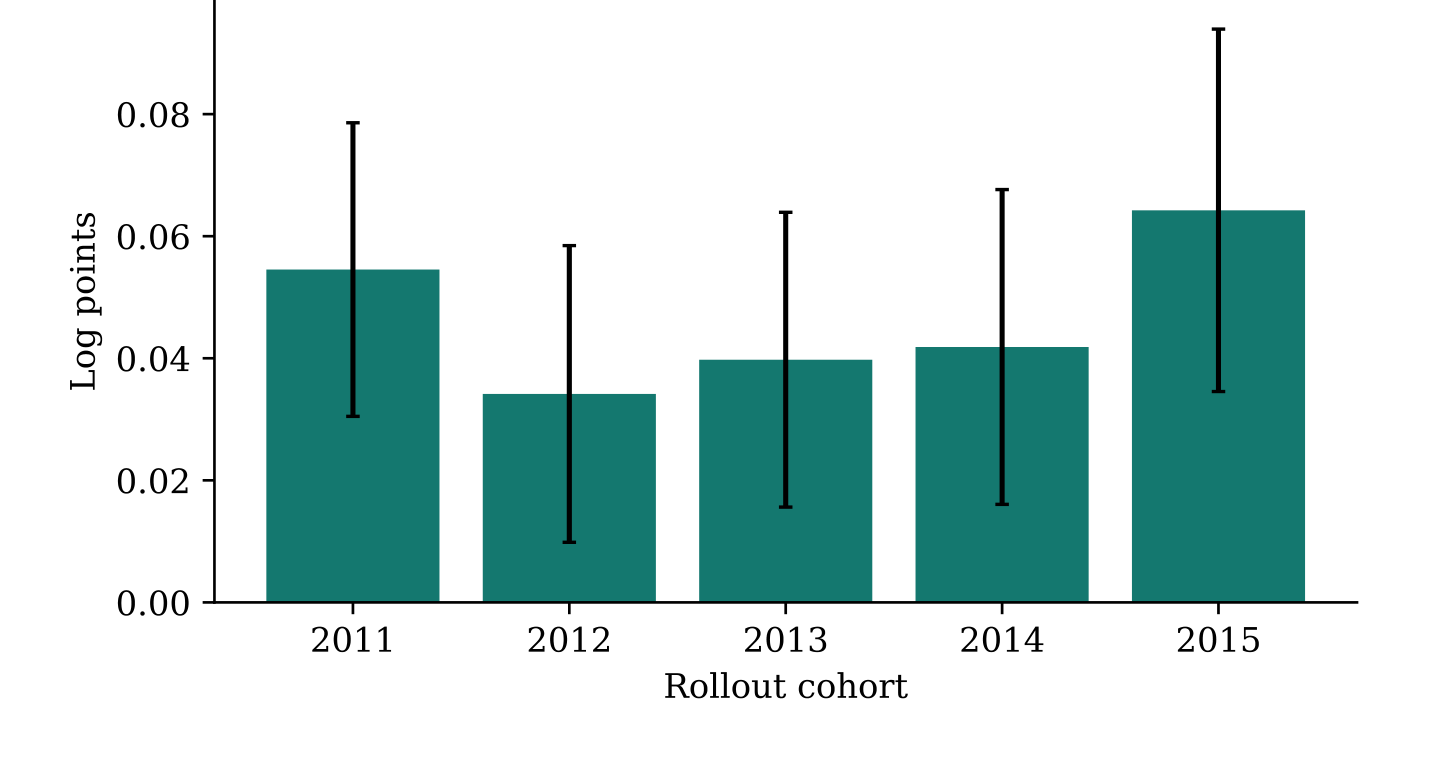
\includegraphics[height=0.60\textheight,keepaspectratio]{figures-slides/fig3_cohorts.png}
  \TakeawayWithNav{\textbf{Identification:} similar signs across cohorts do not establish parallel untreated trends.}
  \BackButton{main:eventstudy}
\end{frame}

% ---- A4. Placebo ----
\begin{frame}{The placebo table and prose point in different directions}
  \hypertarget{app:placebo}{}%
  \framesubtitle{Pre-treatment sample; rollout years permuted across municipalities}
  % Exact Table 3 cells, p. 8.
  {\centering\large
  \begin{tabular}{lc}
    \toprule
      & Pre-period placebo \\
    \midrule
    Permuted broadband & \ResPlacebo \\
                       & (\ResPlaceboSE) \\
    \bottomrule
  \end{tabular}\par}
  \medskip
  \begin{itemize}\setlength{\itemsep}{0.50em}
    \item The coefficient-to-SE ratio is about $-2$ using rounded reported entries
    \item The prose calls the estimate statistically indistinguishable from zero
    \item The source provides no exact $p$-value or confidence interval
  \end{itemize}
  \TakeawayWithNav{\textbf{Conflict:} the estimate is about two standard errors from zero, contrary to the prose.}
  \BackButton{main:eventstudy}
\end{frame}

% ---- A5. Headline source conflicts ----
\begin{frame}{Two numerical inconsistencies require correction}
  \hypertarget{app:sourceconflicts}{}%
  \framesubtitle{Narrative prose versus exact table cells}
  {\centering\small
  \begin{tabular}{lll}
    \toprule
    Quantity & Narrative source & Exact table source \\
    \midrule
    Headline magnitude & Abstract: 34\%; text: 3.4\% & Table 2: \ResBaseline\ log points \\
    Region-trend estimate & Section 6.1: 0.024 & Table 2: \ResTrends \\
    \bottomrule
  \end{tabular}\par}
  \medskip
  \begin{itemize}\setlength{\itemsep}{0.54em}
    \item The talk reports the coefficient's table unit: log points
    \item The main result table uses exact Table 2 cells in every specification
    \item A 0.034 log-point difference is approximately 3.4\%, not 34\%
  \end{itemize}
  \TakeawayWithNav{\textbf{Correction:} exact cells support a 3.4\% headline; both narrative values need revision.}
  \BackButton{main:estimates}
\end{frame}

% ---- A6. Robustness ----
\begin{frame}{Table 5 is stable but not self-consistent}
  \hypertarget{app:robustness}{}%
  \framesubtitle{Exact reported cells, paper p. 9}
  {\centering\small
  \begin{tabular}{lccc}
    \toprule
      & Region trends & No controls & Drop 2011--12 \\
    \midrule
    Broadband & \ResTrends*** & \ResBaseline*** & \ResDropEarly*** \\
              & (\ResTrendsSE) & (\ResBaselineSE) & (\ResDropEarlySE) \\
    \bottomrule
  \end{tabular}\par}
  \medskip
  \begin{itemize}\setlength{\itemsep}{0.54em}
    \item \RunIn{Stable pattern:} reported coefficients range from \ResTrends\ to \ResDropEarly
    \item \RunIn{Header--note conflict:} ``No controls'' versus ``full control set''
    \item \RunIn{Prose--table conflict:} 0.024 versus \ResTrends\ for region trends
  \end{itemize}
  \TakeawayWithNav{\textbf{Reading:} the coefficient range is narrow, but the source labels need correction.}
  \BackButton{main:estimates}
\end{frame}

% ---- A7. Inference ----
\begin{frame}{Municipal assignment calls for municipal-level inference}
  \hypertarget{app:inference}{}%
  \framesubtitle{Treatment timing varies across \ResMunicipalities\ municipalities}
  {\centering\large
  \begin{tabular}{lcc}
    \toprule
      & Firm-clustered & Municipality-clustered \\
    \midrule
    Broadband & \ResBaseline & \ResMunicipalCluster \\
              & (\ResBaselineSE) & (\ResMunicipalClusterSE) \\
    \bottomrule
  \end{tabular}\par}
  \medskip
  \begin{itemize}\setlength{\itemsep}{0.56em}
    \item The baseline clusters by firm, below the municipal assignment level
    \item Table 2 column (4) reports the assignment-aligned alternative
    \item The point estimate is unchanged and the reported SE rises to \ResMunicipalClusterSE
  \end{itemize}
  \TakeawayWithNav{\textbf{Inference:} clustering changes uncertainty, not the concern about selected timing.}
  \BackButton{main:estimates}
\end{frame}

% ---- A8. Model derivation ----
\begin{frame}[t]{Larger gains require tasks to switch providers}
  \hypertarget{app:modelderivation}{}%
  \framesubtitle{Paper Proposition 1 and proof, pp. 2--3}
  \medskip
  \[
    \underbrace{\kappa_1p}_{\text{remote cost after}}
      \leq
    \underbrace{\phi w}_{\text{quality-adjusted in-house cost}}
      <
    \underbrace{\kappa_0p}_{\text{remote cost before}}
  \]
  \[
    G(\theta_i)=\eta\ln[1+(\phi-1)\theta_i],
    \qquad
    G'(\theta_i)=\frac{\eta(\phi-1)}{1+(\phi-1)\theta_i}>0
  \]
  \begin{itemize}\setlength{\itemsep}{0.58em}
    \item Before arrival, communication-intensive tasks remain in-house
    \item After arrival, the same tasks switch to specialized remote providers
    \item The derivative is positive because $\eta>0$ and $\phi>1$
    \item \RunIn{Scope:} the heterogeneity prediction is conditional on this switch
  \end{itemize}
  \BackButton{main:model}
\end{frame}

% ---- A9. Mechanism interpretation ----
\begin{frame}{The interaction is consistent with, not unique to, outsourcing}
  \hypertarget{app:mechanism}{}%
  \framesubtitle{What Table 4 observes and what it leaves unmeasured}
  \medskip
  \begin{itemize}\setlength{\itemsep}{0.68em}
    \item \RunIn{Observed:} a positive interaction with 2008 communication intensity
      \begin{itemize}
        \item one SD adds \ResCommSDGap\ log points
      \end{itemize}
    \item \RunIn{Predicted:} the task model gives the same positive sign
      \begin{itemize}
        \item the switching case makes $G'(\theta_i)>0$
      \end{itemize}
    \item \RunIn{Unobserved:} remote procurement, task reorganization, and channel-specific inputs
    \item \RunIn{Alternative:} other firm traits can generate the same pattern
  \end{itemize}
  \bigskip
  \textbf{Discriminating evidence:} direct measures of sourcing before and after arrival.
  \BackButton{main:heterogeneity}
\end{frame}

% ---- A10. Policy arithmetic ----
\begin{frame}{The six-year payback is not traceable from the reported inputs}
  \hypertarget{app:policy}{}%
  \framesubtitle{Paper Section 7, pp. 8--9}
  \medskip
  \begin{itemize}\setlength{\itemsep}{0.68em}
    \item \RunIn{Claimed flow:} \ResPolicyValue\ per year against \ResPolicyCost\ in construction
    \item \RunIn{Estimate:} a productivity association among sample survivors
    \item \RunIn{Missing inputs:} firm value added, program coverage, and maintenance costs
    \item \RunIn{Missing assumptions:} causality, persistence, discounting, and incidence
    \item \RunIn{Unit problem:} gross output is not a fiscal return
  \end{itemize}
  \bigskip
  \textbf{Conclusion for this talk:} the payback and cost-effectiveness claims are excluded.
  \BackButton{main:conclusion}
\end{frame}

\end{document}
